%% Creator: Inkscape inkscape 0.48pre0, www.inkscape.org
%% PDF/EPS/PS + LaTeX output extension by Johan Engelen, 2010
%% Accompanies image file 'frameworkOverview' (pdf, eps, ps)
%%
%% To include the image in your LaTeX document, write
%%   \input{<filename>.tex}
%%  instead of
%%   \includegraphics{<filename>.pdf}
%% To scale the image, write
%%   \def{\svgwidth}{<desired width>}
%%   \input{<filename>.tex}
%%  instead of
%%   \includegraphics[width=<desired width>]{<filename>.pdf}

\begingroup
  \makeatletter
  \providecommand\color[2][]{%
    \errmessage{(Inkscape) Color is used for the text in Inkscape, but the package 'color.sty' is not loaded}
    \renewcommand\color[2][]{}%
  }
  \providecommand\transparent[1]{%
    \errmessage{(Inkscape) Transparency is used (non-zero) for the text in Inkscape, but the package 'transparent.sty' is not loaded}
    \renewcommand\transparent[1]{}%
  }
  \providecommand\rotatebox[2]{#2}
  \ifx\svgwidth\undefined
    \setlength{\unitlength}{348.6875pt}
  \else
    \setlength{\unitlength}{\svgwidth}
  \fi
  \global\let\svgwidth\undefined
  \makeatother
  \begin{picture}(1,1.00224054)%
    \put(0,0){\includegraphics[width=\unitlength]{frameworkOverview}}%
    \put(0.16421171,0.95050233){\makebox(0,0)[lb]{\smash{Client}}}%
    \put(0.23751574,0.95050233){\makebox(0,0)[lb]{\smash{A}}}%
    \put(0.26711216,0.95050233){\makebox(0,0)[lb]{\smash{(ServiceAPI)}}}%
    \put(0.30006286,0.8803048){\makebox(0,0)[lb]{\smash{HTTPRequest}}}%
    \put(0.59347745,0.95050233){\makebox(0,0)[lb]{\smash{Client}}}%
    \put(0.66678149,0.95050233){\makebox(0,0)[lb]{\smash{B}}}%
    \put(0.69534621,0.95050233){\makebox(0,0)[lb]{\smash{(ServiceAPI)}}}%
    \put(0.72864146,0.8803048){\makebox(0,0)[lb]{\smash{HTTPRequest
Client-side}}}%
    \put(0.01425655,0.82075004){\makebox(0,0)[lb]{\smash{Server-side}}}%
    \put(0.35830986,0.78110709){\makebox(0,0)[lb]{\smash{WebAPI
(django/piston)}}}%
    \put(0.03850488,0.68743296){\makebox(0,0)[lb]{\smash{ROS}}}%
    \put(0.18966315,0.78396639){\makebox(0,0)[lb]{\smash{Service}}}%
    \put(0.20686279,0.68679629){\rotatebox{90}{\makebox(0,0)[lb]{\smash{get
post}}}}%
    \put(0.53012273,0.78396639){\makebox(0,0)[lb]{\smash{Environment}}}%
    \put(0.56400981,0.68687659){\rotatebox{90}{\makebox(0,0)[lb]{\smash{delete
get
post}}}}%
    \put(0.74560508,0.78396639){\makebox(0,0)[lb]{\smash{Task}}}%
    \put(0.74972911,0.68679629){\rotatebox{90}{\makebox(0,0)[lb]{\smash{get
delete}}}}%
    \put(0.20651893,0.44619976){\rotatebox{90}{\makebox(0,0)[lb]{\smash{getService}}}}%
    \put(0.25750011,0.37852312){\rotatebox{90}{\makebox(0,0)[lb]{\smash{addEnvironment}}}}%
    \put(0.3517854,0.33945375){\rotatebox{90}{\makebox(0,0)[lb]{\smash{removeEnvironment}}}}%
    \put(0.18932703,0.30110136){\makebox(0,0)[lb]{\smash{ServerNode}}}%
    \put(0.19139192,0.2496725){\makebox(0,0)[lb]{\smash{ROSLaunch
(scriptapi)}}}%
    \put(0.60652352,0.38402661){\rotatebox{90}{\makebox(0,0)[lb]{\smash{getEnvironment}}}}%
    \put(0.64893399,0.46669376){\rotatebox{90}{\makebox(0,0)[lb]{\smash{addTask}}}}%
    \put(0.70036399,0.46037865){\rotatebox{90}{\makebox(0,0)[lb]{\smash{addNode}}}}%
    \put(0.74938497,0.47219725){\rotatebox{90}{\makebox(0,0)[lb]{\smash{getTask}}}}%
    \put(0.80608043,0.42762439){\rotatebox{90}{\makebox(0,0)[lb]{\smash{removeTask}}}}%
    \put(0.55724444,0.34931645){\makebox(0,0)[lb]{\smash{isActive
EnvironmentNode}}}%
    \put(0.81166623,0.30110222){\makebox(0,0)[lb]{\smash{A}}}%
    \put(0.64854109,0.2496725){\makebox(0,0)[lb]{\smash{ROSLaunch
(scriptapi)}}}%
    \put(0.18398902,0.06475908){\makebox(0,0)[lb]{\smash{Node}}}%
    \put(0.25075396,0.06475908){\makebox(0,0)[lb]{\smash{A/a}}}%
    \put(0.47005175,0.06475908){\makebox(0,0)[lb]{\smash{Node}}}%
    \put(0.53681669,0.06475908){\makebox(0,0)[lb]{\smash{A/b}}}%
    \put(0.7557689,0.06475908){\makebox(0,0)[lb]{\smash{Node}}}%
    \put(0.82253384,0.06475908){\makebox(0,0)[lb]{\smash{A/c}}}%
    \put(0.92785709,0.45130175){\rotatebox{90}{\makebox(0,0)[lb]{\smash{Namespace}}}}%
    \put(0.92785709,0.58448634){\rotatebox{90}{\makebox(0,0)[lb]{\smash{A}}}}%
  \end{picture}%
\endgroup
